\documentclass[convert={density=300,size=1920x1080,outext=.png}]{standalone}
%\documentclass{standalone}
\usepackage{tikz,pgfplots}
\usepackage{xcolor}

\renewcommand{\familydefault}{\sfdefault}


\usepackage{sansmath} % sans serif math
\sansmath % if you use it globaly

\usetikzlibrary{mindmap, shadows}
\usetikzlibrary{decorations.pathreplacing}

\begin{document}

	\definecolor{border_color}{RGB}{80,116,172}
	\definecolor{fill_color}{RGB}{162,203,240}
	\definecolor{dot_color}{RGB}{60,60,60}

    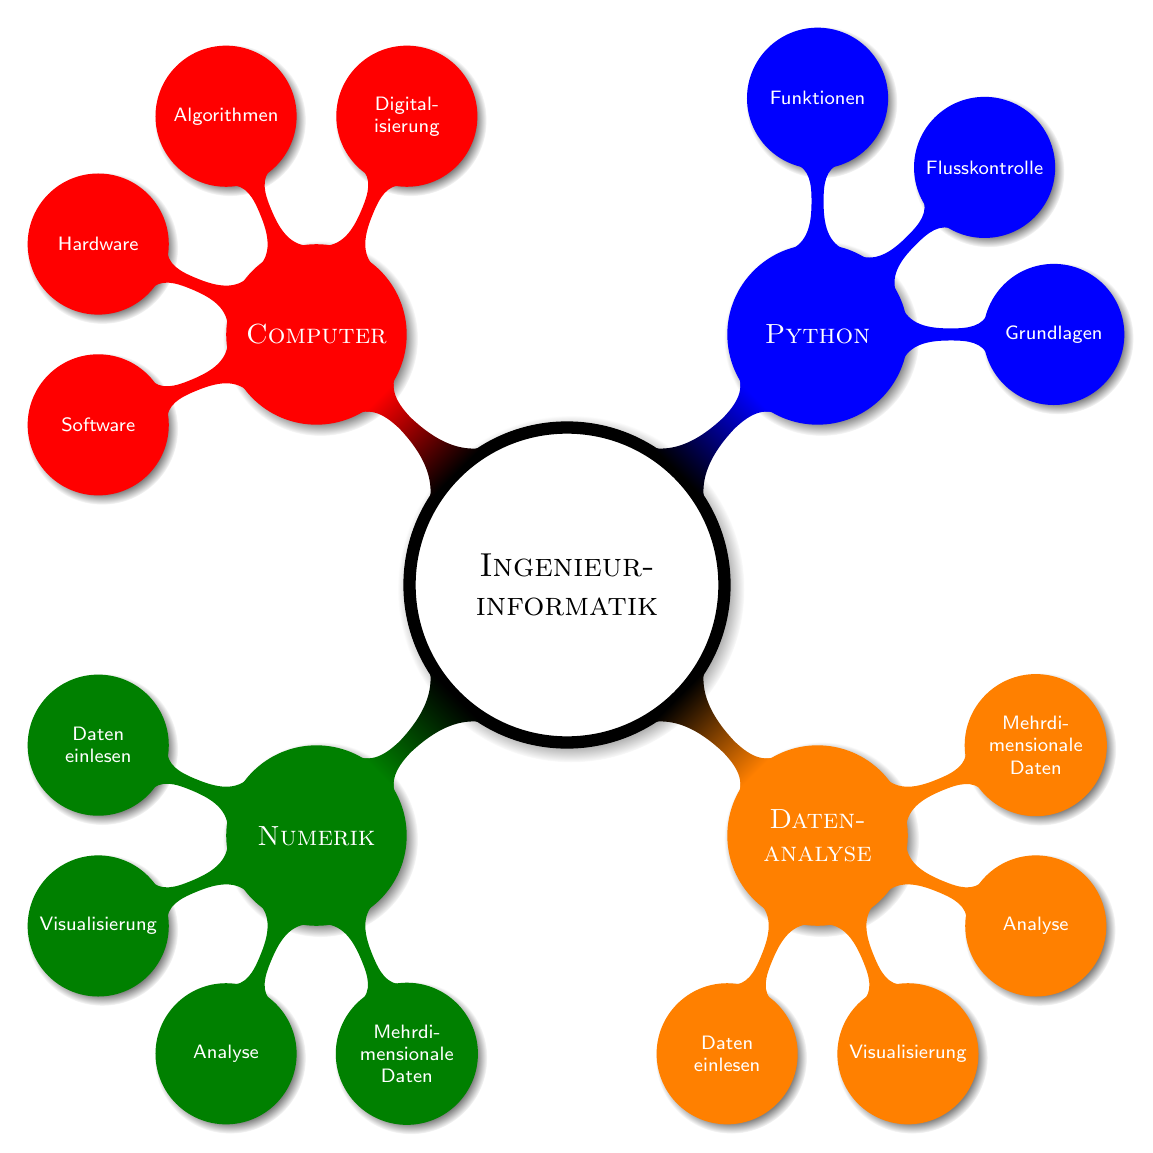
\begin{tikzpicture}[mindmap, font=\sffamily]
  		\begin{scope}[every node/.style={concept, circular drop shadow, execute at begin node=\hskip0pt}, root concept/.append style={concept color=black, fill=white, line width=1ex, text=black, font=\large\scshape}, text=white, computational problems/.style={concept color=red,faded/.style={concept color=red!50}}, computational models/.style={concept color=blue,faded/.style={concept color=blue!50}}, measuring complexity/.style={concept color=orange,faded/.style={concept color=orange!50}}, solving problems/.style={concept color=green!50!black,faded/.style={concept color=green!50!black!50}}, grow cyclic, level 1/.append style={level distance=4.5cm,sibling angle=90,font=\scshape}, level 2/.append style={level distance=3cm,sibling angle=45,font=\scriptsize}] 
\node [root concept] {Ingenieurinformatik} % root
	  child [solving problems] { node {Numerik} 
	  	child { node {Daten einlesen} } 
	  	child { node {Visualisierung} } 
	  	child { node {Analyse} } 
	  	child { node {Mehrdimensionale Daten} } 
	  }
	  child [measuring complexity] { node {Datenanalyse} 
	  	child { node {Daten einlesen} } 
	  	child { node {Visualisierung} } 
	  	child { node {Analyse} } 
	  	child { node {Mehrdimensionale Daten} } 
	  }
	  child [computational models] { node {Python} 
	  	child { node {Grundlagen} } 
	  	child { node {Flusskontrolle} } 
	  	child { node {Funktionen} } 	  	
	  }
      child [computational problems] { node {Computer}
        child { node {Digitalisierung} }
        child { node {Algorithmen} }
        child { node {Hardware} }
        child { node {Software} }
      }
	  ;

  		\end{scope}
	\end{tikzpicture}

\end{document}